\documentclass[12pt,a4paper]{article}
\usepackage[utf8]{vietnam}
\usepackage{amsmath}
\usepackage{amsfonts}
\usepackage{amssymb}
\usepackage{array}
\usepackage[left=2cm,right=2cm,top=2cm,bottom=2cm]{geometry}
\author{Huu Tai}
\usepackage{indentfirst}
\usepackage{footnote}
\usepackage{graphicx}
\begin{document}
\section{Vấn đề về đánh giá tự động cho bài tập lập trình}
\subsection{Giới thiệu}
Trong thời kỳ ngày càng phát triển của mạng internet thì việc chấm điểm tự động cho các bài tập lập trình ngày càng trở nên quan trọng hơn đặc biệt là khi có sự xuất hiện của các khóa học trực tuyến ngày càng phổ biến hoặc là các lớp học có sinh viên tham gia với số lượng lớn. Đánh giá là một phần không thể thiếu trong giáo dục và thường được sử dụng để đánh giá và cung cấp kết quả cho sinh viên tham gia vào môn học. Đồng thời dựa vào các kết quả đánh giá sau môn học của sinh viên mà giáo viên có thể xác định liệu chương trình giảng dạy có đáp ứng được nhu cầu cần thiết của sinh viên hay không.\newline  
\indent Trong lĩnh vưc giáo dục tâm lý, người ta đã chứng minh rằng hầu hết sinh viên thường hướng những nỗ lực của họ dựa trên kết quả của các bài kiểm tra sau khi được đánh giá và ảnh hưởng của các kết quả đó đến kết quả cuối cùng của khóa học. Đánh giá liên tục trong một khóa học lập trình đảm bảo rằng sinh viên hoàn thành đủ các bài kiểm tra cũng như nhận lại phan hồi về kết quả của các bài kiểm tra đó. Tuy nhiên việc đánh giá kết quả một cách thủ công cho một lớp học đòi hỏi rất nhiều công sức và rất dễ bị lỗi và việc đấy càng được thể hiện rõ ràng khi số lượng sinh viên trong một lớp học tăng lên (Ví dụ, các khóa học lập trình khác nhau trên edX plat-form có hơn 150000 sinh viên đăng ký trên toàn thế giới [1]), điều đó làm cho việc chấm điểm nhanh chóng cho tất cả các bài tập của sinh viên trở nên khó khăn hơn nhiều. Nhiều khóa học trực tuyến áp dụng phản hồi ngang hàng [2], nhưng loại phản hồi này không đáp ứng được như mong muốn. Sinh viên phải chờ hàng giờ để nhận được phản hồi và giáo viên hướng dẫn chỉ có kiến thức hạn chế về các quy trình đánh giá ngang hàng không có cấu trúc này. Lúc đó việc đánh giá kết quả của sinh viên đòi hỏi phải được giới hạn hoặc hợp lý hóa theo một cách nào đó.\newline
\indent Trong thực tế hai giáo viên chấm cùng một môn rất hiếm khi áp dụng cùng một tiêu chí đánh giá trong mọi trường hợp. Điều này là không công bằng với sinh viên bởi vì điều đó có nghĩa là điểm đánh giá của học sinh có thể phụ thuộc vào từng giải pháp đánh giá của giáo viên mà không chỉ dựa vào giải pháp của học sinh. Và việc này càng xảy ra phổ biến trong việc đánh giá các bài tập lập trình.\newline
\indent Thông thường sẽ có vô số giải pháp khả thi cho cùng một vấn đề vì có thể có thể có các biến thể trong các lập trình do đó một mẫu đánh giá sẽ cũng cấp hướng dẫn cho người đánh giá nhưng sẽ không bao quát hết tất các cả trường hợp. Điều đó đòi hỏi phải có một công cụ giúp đánh giá các bài kiểm tra một cách tự động và hơn hết là đảm bảo đánh giá một cách công bằng, khách quan và được áp dụng như nhau cho tất cả học sinh. Thách thức này đã dẫn đến sự phát triển của các công cụ chấm điểm tự động.\newline
\indent Hiện nay đã có nhiều hệ thống đánh đánh giá tự động tồn tại những hàng năm vẫn có rất nhiều hệ thống đánh giá khác được tạo ra. Các hệ thống đã tồn tại đều đã đáp ứng hầu hết các nhu cầu về đánh giá.
Một lý do rõ ràng cho sự đa dạng của các công cự đó là tuổi thọ và tính khả dụng của nó. Các công cụ đánh giá được tạo ra như là một phần của các khóa học. Nó giúp cho việc đánh giá kết quả của toàn bộ học viên trong khóa học một cách nhanh chóng nhưng không phù hợp để phân phối rộng rãi cho các khóa học khác. Thông thường các công cụ được các giảng viên sử dụng để hỗ trợ trong việc đánh giá các bài tập lập trình vì vậy rất ít các công cụ xuất hiện dưới dạng phần mềm được hỗ trợ và sử dụng rộng rãi. Vì vậy các các công cụ đánh giá tự động thường được lặp đi lặp lại rất nhiều đồng thời có rất ít các công cụ đáng giá tự động được sử dụng một cách rộng rãi và phổ biến.\newline
\indent  Trong bài báo cáo này sẽ trình bày và so sánh các công cụ được sử dụng để chấm điểm tự động cho các bài tập lập trình.\newline
\subsection{Các lỗi phần mềm}
Trước khi trình bày về các kỹ thuật và hệ thống tự động đánh giá tôi muốn giới thiệu các lỗi thường được xem xét đến bởi các kỹ thuật này. Lỗi phần mềm được định nghĩa là tạo ra kết quả sai hoặc thực hiện một hành động theo cách không lường trước được. Lỗi phần mềm được phân loại thành các lỗi như: Lỗi cú pháp, lỗi logic và lỗi thời gian chạy.
\begin{itemize}
\item[-] \textbf{Lỗi cú pháp}: Lỗi này được phát hiện khi cú pháp không chính xác trong ngôn ngữ lập trình, ví dụ như cấu trúc chương trình không chính xác, các từ sai, thiếu dấu chấm phẩy. Loại lỗi này có thể được trình biên dịch ngôn ngữ lập trình phát hiện trong khi biên dịch mã phần mềm. Lỗi này là lỗi dễ phát hiện và sửa nhất vì hầu hết các trình biên dịch được sử dụng ngày nay.\newline
\item[-] \textbf{Lỗi logic}: Khi mắc lỗi này phần mềm biên dịch vẫn chạy tốt nhưng đầu ra của phần mềm bị sai do nhiều lý do như sai về yêu cầu hoặc đặc tả, lỗi toán học (chia cho 0). Vì lỗi này không được trình biên dịch phát hiện nên ta cần phát hiện các lỗi này trước khi khởi chạy phần mềm.\newline
\item[-] \textbf{Lỗi thời gian chạy}: Đây là lỗi nâng cao và rất hiếm khi sinh viên bị rơi vào. Lỗi thời gian chạy chỉ xảy ra khi phần mềm đang chạy. Trong thực tế đây là một trong những vấn đề phức tạp nhất để theo dõi và dẫn đến sự cố phần mềm.\newline
\end{itemize}
\subsection{Lợi ích của việc sử dụng đánh giá tự động}
Việc áp dụng các hệ thống tự động đánh giá vào trong các khóa học đem lại các lợi ích sau:
\begin{itemize}
\item[-] \textbf{Tốc độ}: Giúp cho việc đánh giá nhanh hơn nhiều và sinh viên sẽ nhận được kết quả ngay sau kỳ thi. Khi sử dụng đánh giá thủ công thì sinh viên cần chờ một khoảng thời gian rất lâu để nhận được kết quả đánh giá của bài kiểm tra. Ngược lại với hệ thống đánh giá tự động, các sinh viên có thể tự đánh giá bài kiểm tra của mình, biết điểm của họ và sửa lỗi của chính họ.
\item[-] \textbf{Công bằng}: Các lỗi tương tự sẽ được đánh giá như nhau và giáo viên sẽ không ảnh hưởng đến việc chấm điểm.
\item[-] \textbf{Độc lập}: Việc đánh giá một bài kiểm tra không bị ảnh hưởng từ kết quả của các bài kiểm tra trước đó. Trong đánh giá thủ công, một bài kiểm tra lúc trước có kết quả không tốt có thê khiến giá viên chủ quan coi bài kiểm tra tiếp theo là không tốt.
\end{itemize}
\section{Kỹ thuật sử dụng trong các hệ thống đánh giá tự động và các công cụ}
Hiện nay có rất nhiều hệ thống đánh giá tự động đang tồn tại nhưng để đảm bảo rằng các hệ thống đó đem lại kết quả đánh giá một cách chính xác là một điều khó khăn. Một trong những vấn đề quan trọng ảnh hưởng đến kết quả đánh giá của một hệ thống đó là việc xây dựng các bộ kiểm thử có chất lượng cao. Trên thực tế, việc cung cấp các bộ kiểm thử bằng cách thủ công là một quá trình rất chậm và tốn thời gian, điều này dẫn đến việc tạo ra các bộ kiểm thử không hiệu quả và không đầy đủ. Điều này dẫn đến chất lượng của hệ thống đánh giá bị ảnh hưởng.\newline
\indent Công cụ tạo bộ kiểm thử tự động ra đời để giải quyết vấn đề nói trên. Với việc tự động sinh ra các bộ kiểm thử có độ bao phủ cao với các tiêu chí kiểm thử nhằm phát hiện các lỗi sâu trong các hệ thống phần mêm phức tạp, công cụ này đã giúp cải thiện độ chính xác cao của các hệ thống đánh giá tự động. Symbolic execution là một trong các kỹ thuật nổi tiếng được sử dụng trong các công cụ tự động sinh bộ kiểm thử. Trong phần tiếp theo chúng ta sẽ tìm hiểu kỹ hơn về kỹ thuật này và một số công cụ hỗ trợ việc tự động sinh bộ kiểm thử.
\subsection{Symbolic execution}
\subsubsection{Giới thiệu}
Trong hoạt động kiểm thử phần mềm, các ca kiểm thử thường được tạo ra một cách thủ công, gây tốn kém về chi phí cũng như thời gian để hoàn thành công đoạn này. Thực thi tượng trưng (Symbolic execution) được biết đến là một kỹ thuật nổi tiếng với khả năng tự động sinh những bộ test case có độ bao phủ cao với các tiêu chí kiểm thử nhằm phát hiện những lỗi sâu trong các hệ thống phần mềm phức tạp.\newline
\indent Hiện nay có rất nhiều công cụ nền tảng phục vụ cho hoạt động kiểm thử phần mềm như JUnit cho ngôn ngữ Java, Nunit, VSUnit cho .NET để thực thi các ca kiểm thử ở mức đơn vị. Tuy nhiên các công cụ kiểm thử này không hỗ trợ việc sinh tự động các ca kiểm thử đơn vị. Viết các ca kiểm thử là một công việc nặng nhọc và tốn nhiều công sức. Có nhiều phương pháp khác nhau hỗ trợ việc sinh tự động các ca kiểm thử (Test case) giúp giảm chi phí và thời gian thực hiện đã được nghiên cứu và đưa ra như: Dựa trên mô hình (Model Checking), kiểm thử ngẫu nhiên (Random Testing [1]). Nhưng hạn chế của nó là kiểm tra cùng 1 hành vị thực thi của chương trình nhiều lần với những đầu vào khác nhau và chỉ có thể kiểm tra được một số trường hợp thực thi của chương trình. Thêm vào đó, kiểm thử ngẫu nhiên khó xác định được khi nào việc kiểm thử nên được dừng lại và nó không biết tại điểm nào không gian trạng thái đã được thám hiểm hết. Để xác định khi nào việc kiểm thử dừng lại thì hệ thống kiểm thử ngẫu nhiên được kết hợp với các tiêu chuẩn an toàn [3]. Để khắc phục những hạn chế của kiểm thử ngẫu nhiên, phương pháp thực thi tượng trưng xây dựng các ràng buộc trên các giá trị tượng trưng và giải các ràng buộc đó để sinh ra các giá trị đầu vào cho chương trình mà nó có thể bao phủ tất cả các dòng lệnh cũng như các nhánh thực thi của chương trình.\newline
\indent Ý tưởng của thực thi tượng trưng đã được đề xuất bởi King [Comm. ACM 1976], Clarke [IEEE TSE 1976] nhưng việc hiện thực ý tưởng mới chỉ được thực hiện trong những năm gần đây qua tiến bộ đáng kể trong lý thuyết giải các ràng buộc (Constrain satisfiability) [11] và các tiếp cận mở rộng thực thi tượng trưng động (Dynamic symbolic execution), một kỹ thuật kết hợp giữa các giá trị cụ thể và giá trị tương trưng cho các giá trị đầu vào.\newline
\subsubsection{Tổng quan về kỹ thuật Symbolic execution}
Ý tưởng chính của Symbolic execution là thực thi chương trình với các giá trị tượng trưng (Symbolic value) thay vì các giá trị cụ thể (concrete value) của các tham số đầu vào. Kết quả là giá trị đầu ra được tính toán bởi chương trình và được biểu diễn bởi bởi một biểu thức tượng trưng. Trong kiểm thử phần mềm, kỹ thuật Symbolic execution được sử dụng để sinh dữ liệu kiểm thử cho mỗi đường thực thi khác nhau của chương trình. Ví dụ trong hình 1 minh họa Symbolic execution.\newline
\indent Trong quá trình thực thi tượng trưng, việc đi theo một nhánh cụ thể nào đó không phụ thuộc vào các giá trị của các tham số đầu vào. Tại tất cả các điểm rẽ nhánh, tất cả các nhánh sẽ được xem xét và kiểm tra nhằm định hướng cho thực thi tiếp theo của chương trình. Với những chương trình ở dạng đơn giản có hại loại thực thi chủ yếu: đó là câu lệnh gán và câu lệnh rẽ nhánh. Tại các câu lệnh gán, giá trị tượng trưng của biến chương trình cũng như các tham số đầu vào có liên quan đến câu lệnh đó được tính toán và cập nhập lại, còn tại các điểm rẽ nhánh, chương trình sẽ điều khiển thực thi theo cả hai nhánh tương ứng đồng thời ràng buộc đường đi (Path condition) tương ứng với hai nhánh sẽ được tạo ra. Một ràng buộc là một biểu thức điều kiện tương ứng với giá trị true, ràng buộc kia tương ứng với giá trị false của biểu thức ràng buộc. Các ràng buộc này sẽ được cập nhập vào đường đi tương ứng với nhánh đó. Các ràng buộc này sẽ được xen xét bởi một bộ giải ràng buộc để đánh giá xem đường đi tiếp theo có khả thi không hay nói một cách khác là kiểm tra xem có tồn tại bộ giá trị thõa mãn ràng buộc này hay không. Nếu không thõa màn thì ràng buộc sẽ đánh giá là sai, khi đó Symbolic execution sẽ dừng hoặc quay lui thực thi theo nhánh khả thi.\newline
\begin{figure}[ht]
\begin{center}
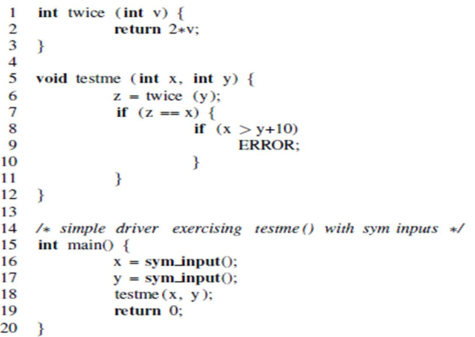
\includegraphics{hinhanh/hinh1}
\end{center}
\caption{Ví dụ cho symbolic execution}
\end{figure}
\indent Các ràng buộc đường đi được tạo ra bằng cách thu gom các điều kiện trên đường đi tương ứng. Giải các ràng buộc này sẽ sinh ra các giá trị cụ thể cho các tham số đầu vào tương ứng với từng nhánh thực thi của chương trình.\newline
\indent Tất cả các đường thực thi của chương trình có thể biểu diễn bởi một cấu trúc cây gọi là cây thực thi (Tree execution). Hình 2 là cây thực thi tượng trưng cho hàm testme() trong hình 1. Các cạnh của cây biểu diễn cho sự chuyển đổi từ trạng thái này sang trạng thái khác. Với ví dụ trên phương thức testme() trong hình 1 sẽ có cây thực thi mô tả những đường thực thi của chương trình với các biến đầu vào là {x=0, y=1}, {x=2, y=1}, {x=30, y=15}, mục tiêu là sinh ra tập các ca kiểm thử thõa mãn thực thi cho tất cả các nhánh của chương trình phụ thuộc vào giá trị tượng trưng của các tham biến đầu vào nhiều nhất có thể trong một khoảng thời gian nhất định đảm báo khám phá chính xác tất cả các đường thực thi bởi một lần duy nhất với những giá trị đầu vào đã cho.\newline
\begin{figure}[ht]
\begin{center}
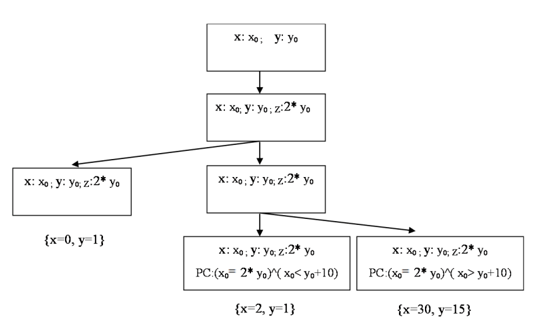
\includegraphics{hinhanh/hinh2}
\end{center}
\caption{Cây Symbolic execution tương ứng với hàm testme() trong ví dụ 1}
\end{figure}
\indent Bắt đầu thực thi tượng trưng hàm testme() bằng việc gán giá trị cho các tham số đầu vào x và y lần lượt là $x_0$, $y_0$. Khởi tạo PC (Path condition) nhận giá trị là true, tới câu lệnh rẽ nhánh $if(2*y_0=x_0)$ hai nhanh của chương trình tương ứng đều được thực thi với các giá trị tương ứng là $x_0$ và $y_0$. Tại đây biểu thức điều kiện rẽ nhánh là $2*y_0=x_0$ và $!(2*y_0=x_0)$ được bổ sung và PC theo hai nhánh khác nhau. Sau khi thực thi câu lệnh $if(2*y_0=x_0)$ hàm testme() được thực thi theo nhánh mà tồn tại bộ giá trị x,y thõa mãn. Tương tự như trên, khi gặp câu lệnh $if(x_0>y_0+10)$ PC theo hai nhánh tương ứng sẽ được cập nhập bổ sung là $(2*y_0=x_0)$ \^{} $(x_0>y_0+10)$ và $(2*y_0=x_0)$\^{}$(x_0<y_0+10)$. Tại mỗi điểm rẽ nhánh PC sẽ được cập nhập và một thủ tục quyết định bằng bộ xử lý ràng buộc sẽ được sử dụng để xác định xem nhánh tương ứng với PC đó có khả thi hay không để điều hướng thực thi hiện thời đi theo nhánh đó. Nếu PC được đánh giá là không khả thi thực thi tượng trưng sẽ dừng hoặc quay lui, và thực thi tượng trưng chỉ thực thi chương trình tượng trưng theo nhánh mà PC được đánh giá là khả thi.\newline
\indent Đối với những đoạn mã chứa vòng lặp hoặc lời gọi đệ quy mà đường thực thi là vô hạn và biến điều khiển của vòng lặp hoặc lời gọi đệ quy là tượng trưng. Ví dụ trong hình 3 sẽ là vô hạn đường thực thi với mỗi đường thực thi là 1 dãy tùy ý số lượng giá trị là true và sau cùng là false hoặc là một dãy vô hạn số lần lặp, khi đó PC của đường thực thị là một dãy gồm n giá trị true và sau cùng là false.\newline
\begin{figure}[ht]
\begin{center}
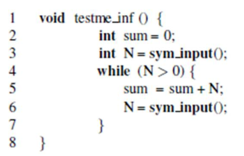
\includegraphics{hinhanh/hinh3}
\end{center}
\caption{Ví dụ cho vòng lặp vô hạn}
\end{figure}
\indent Trên thực tế cần phải thêm các tiêu chí giới hạn cho việc tìm kiếm như thời gian thực thi, giới hạn chiều sâu của đường thực thi hoặc số lượng các vòng lặp lồng nhau.\newline
\indent Nhược điểm chính của Symbolic execution truyền thống là không thể sinh dữ liệu test nếu không giải được biểu thức ràng buộc đường thực thi. Ví dụ nếu ta thay hàm twice() ở hình 1 bằng hàm twice() ở hình 4 sau khi thực hiện câu lệnh dòng 7 thì thực thi tượng trưng sẽ cho ra hai ràng buộc mới bổ sung $x_0$\#$y_0$*$y_0$\%50 và $x_0=y_0$*$y_0$\%$50$ và khi bộ giải ràng buộc không giải được ràng buộc trên thực thi tượng trưng sẽ thất bại trong việc sinh các dữ liệu kiểm thử cho chương trình sau khi đã được sửa đổi.\newline
\begin{figure}[ht]
\begin{center}
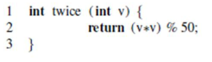
\includegraphics{hinhanh/hinh4}
\end{center}
\caption{Ví dụ cho hàm twice()}
\end{figure}
\subsection{CTGEN}
Trong phần này tôi sẽ trình bày về CTGEN một công cụ tạo thử nghiệm tự động dựa trên kỹ thuật Symbolic execution. Mục tiêu của CTGEN là bao quát moị chi nhánh trong chương trình nhưng đây là một vấn đề không thể giải quyết được, vì vậy trong thực tế CTGEN cố gắng tạo ra thử nghiệm với độ bao phủ cao cho các modul trong các thử nghiệm. Đối với mỗi đơn vị được thử nghiệm, CTGEN thực hiện phân tích biểu tượng và tạo một thử nghiệm theo cú pháp RTTester [13] có thể được biện dịch và thực hiện trực tiếp. Ngoài các biến có kiểu dữ liệu cơ bản, CTGEN còn hỗ trợ các biến có dấu chấm động, con trỏ, cấu trúc và mảng. CTGEN có thể đối phó với các vấn đề điển hình trong C bởi sử dụng con trỏ và mảng. Trong CTGEN các hàm đệ quy, bộ nhớ động, cấu trúc dữ liệu động phức tạp với các con trỏ (lists, stacks,...) và các luồng chương trình đồng thời sẽ không được hổ trợ. CTGEN không kiểm tra modul đang thử nghiệm để tìm lỗi thời gian chạy mà nó giao nhiệm vụ này cho một trình thông dịch trừu tượng khác [21].\newline
\indent CTGEN không dựa vào kiến thức về tất cả các phần của chương trình chẳng hạn như các chức năng thư viện hoặc không xác định. Khi một số công cụ tự động kiểm tra đơn vị khác [25] rơi vào lệnh gọi các sub-function với các giá trị đầu vào cụ thể, nếu một external function xảy ra trên đường dẫn khám, CTGEN sẽ tự động tạo ra một đối tượng giả thay thế external function bởi test stub. Hơn nữa nó sẽ tính toán các giá trị cho dữ liệu trả về stub, các tham số đầu ra và các biến toàn cục có thể được sửa đổi bời stubbed function để đáp ứng điều kiện đường dẫn. Theo cách này, CTGEN cũng có thể mô phỏng hành vi đặc biệt của các external function.\newline
\indent CTGEN được phân biệt với các công cụ khác với các khả năng sau: xử lý các cuộc gọi đến external function bằng các đối tượng giả, con trỏ tượng trưng và xử lý bù trừ, theo dõi yêu cầu. Con trỏ và external function là các thách thức quan trọng nhất đối với các công cụ tạo dữ liệu thử nghiệm và CTGEN là một công cụ có thể xử lý cả hai vấn đề này. \newline
\indent CTGEN được cấu trúc thành hai phần chính: (Hình 5)\newline
\begin{figure}[ht]
\begin{center}
\includegraphics{hinhanh/ctgen}
\end{center}
\caption{Kiến trúc tổng quan của CTGEN}
\end{figure}
\indent Bộ tiền xử lý hoạt động trên mã UUT. Nó bao gồm các chú thích mã tiền xử lý CTGEN, một pluggin GCC biên dịch mã nguồn đã chuẩn bị thành một đặc tả văn bản bao gồm biểu đồ luồng điều khiển (CFG) và thông tin bảng ký hiệu như function signatures, types và variables, trình phân tích cú pháp , chuyển đổi CFG và thông tin bảng ký hiệu thành biễu diễn mô hình trung gian (IMR).\newline
\indent Máy phân tích hoạt động trên IRM, các khối xây dựng của nó và các tương tác của chúng sẽ được mô tả bên dưới. Trình tạo trường hợp kiểm tra tượng trưng (Symbolic Test Case Generator) chịu trách nhiệm cho việc mở rộng các CFG liên quan đến chức năng được kiểm tra và các chức năng phụ của nó. Hơn nữa, nó xử lý việc lựa chọn các đường dẫn, mỗi điểm bắt đầu bằng nút bắt đầu của CFG và chứa các chuyển tiếp chưa được khám phá. Nếu đường dẫn như vậy có thể được tìm thấy, nó được chuyển đến trình thông dịch tượng trưng (Symbolic Interpreter)m, đi qua đường dẫn và tính toán một cách tượng trưng hiệu quả các câu lệnh của nó trong mô hình bộ nhớ. Ngay khi nút tiếp theo trên đường dẫn được bảo vệ bởi một điều kiện không tầm thường (non-trivial), Trình tạo ràng buộc (Constraint Generator) được gọi và giải quyết tất cả các con trỏ và tham chiếu mảng xảy ra trong điều kiện này. Nó cũng chuyển các ràng buộc kết quả cho bộ giải (Solver). CTGEN sử dụng bộ giải SMT, bộ giải này hỗ trợ các kiểu dữ liệu cơ bản, dấu chấm động, mảng và bit vectors. Nếu bộ giải có thể tìm ra giải pháp cho ràng buộc, giải pháp đó được chuyển lại cho trình thông dịch tượng trưng, tiếp tục đi theo con đường đang xét. Mặt khác, nếu ràng là không khả thi hoặc đường dẫn được hoàn thành bộ giải sẽ chuyển kết quả cho bộ tạo trường hợp thử nghiệm tượng trưng. Nó học được từ tính không khả thi và cố gắng tạo ra một đường dẫn khác chứa các chuyển tiếp vẫn chưa được khám phá hoặc cố gắng tiếp tục đường dẫn đã hoàn thành. Khi không tìm thấy đường dẫn như vậy, unit test được tạo dựa trên các giải pháp được thu thập (nếu có) và được lưu trữ trong hệ thống tệp. 
\subsection{PathCrawler}
PATHCRAWLER là một công cụ tạo bộ thử nghiệm cho các chương trình C. Ban đầu được thiết kế để tự động hóa  kiểm tra đơn vị (Unit test) bằng cách tạo đầu vào thử nghiệm để bao phủ toàn bộ cấu trúc của chương trình C đang thử nghiệm.\newline
\indent PATHCRAWLER đã được phát triển tại CEA List từ năm 2002. Trong những năm qua nó đã được mở rộng để xử lý một tập hợp con lớn hơn của các chương trình C và áp dụng cho nhiều vấn đề phân biệt, thường được áp dụng nhiều nhất trong các phần mềm nhúng. Trong năm 2010, nó đã được cung cấp công khai dưới dạng máy chủ thử nghiệm trực tuyến [5], để đánh giá và sử dụng trong giảng dạy.\newline
\indent PATHCRAWLER được xây dựng dựa trên kỹ thuậ Symbolic execution. Người dùng cung cấp các tệp có thể biên dịch có chứa mã chương trình C hoàn chỉnh của hàm được kiểm tra (gọi là f) và tất cả các hàm khác có thể gọi trực tiếp hoặc gián tiếp bởi hàm f. Họ cũng có thể chọn tiêu chí bảo hiểm và bất kỳ giới hạn nào về số lần lặp lại trong các đường dẫn được bảo hiểm cũng như một điều kiện tiên quyết tùy chọn để xác định bối cảnh thử nghiệm. Công việc tạo bộ thử nghiệm bằng PATHCRAWLER gồm hai giai đoạn chính. Trong giai đoạn đầu tiên, PATHCRAWLER trích xuất các đầu vào của f và tạo ra một khai thác thử nghiệm được sử dụng để thực hiện f trên một trường hợp thử nghiệm nhất định. Khai thác thử nghiệm về cơ bản là một phiên bản cụ thể của mã tạo ra dấu vết của đường dẫn được bao phủ bởi mỗi trường hợp thử nghiệm. Các đầu vào được trích xuất bao gồm các tham số chính thức của f và các biến toàn cục không cố định được sử dụng bởi f. Mỗi trường hợp thử nghiệm sẽ cung cấp một giá trị cho mỗi đầu vào này. Giai đoạn này sử dụng nền tảng FRAMA-C [6], được phát triển tại CEA List. Giai đoạn thứ hai tạo ra các đầu vào thử nghiệm để tôn trọng tiêu chí bảo hiểm đã chọn.  Giai đoạn này dựa trên thực thi biểu tượng, tạo ra các ràng buộc đối với các giá trị đầu vào tượng trưng và giải quyết ràng buộc để tìm giải pháp, dưới dạng các giá trị đầu vào cụ thể mới, cho một tập các ràng buộc mới. Thật vậy, thực thi tượng trưng được sử dụng để phân tích dấu vết của đường dẫn thực hiện theo sau khi khai thác thực thi f trên các giá trị đầu vào cụ thể của từng trường hợp thử nghiệm được tạo và tạo ra vị từ đường dẫn xác định các biến đầu vào khiến đường dẫn đó bị che lấp.\newline
\indent Cấu trúc tổng quan của PATCHCRAWLER được minh họa trong Hình 6.
\begin{figure}[ht]
\begin{center}
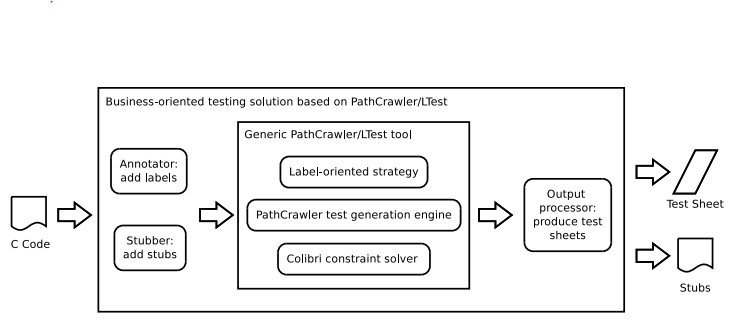
\includegraphics[scale=.7]{hinhanh/pathcrawler}
\end{center}
\caption{Kiến trúc tổng quan của CTGEN}
\end{figure}
Công cụ tạo thử nghiệm chung PATHCRAWLER có ba thành phần chính. Một công cụ kiểm tra đồng thời, PATHCRAWLER, được sử dụng để tạo các trường hợp kiểm thử cho một chương trình C nhất định. Việc tạo các đầu vào kiểm tra cụ thể cho một đường dẫn chương trình nhất định phụ thuộc vào bộ giải ràng buộc, COLIBRI. Cơ chế đặc tả của lable và chiến lược lable-oriented cụ thể cho phép hỗ trợ hiệu quả tiêu chí độ bao phủ thử nghiệm mong muốn được thể hiện dưới dạng lable. Để thích ứng với PATHCRAWLER cho bối cảnh công nghiệp cụ thể, các module bổ sung đã được MERCE, chi nhánh nghiên cứu của đối tác công nghiệp phát triển. Chúng bao gồm ANNOTATOR (thể hiện tiêu chí mục tiêu cụ thể về lable), STUBBER (tạo ra các stubs cần thiết) và PROCESSOR OUTPUT (tạo báo cáo thử nghiệm cần thiết).\newline
\indent PATHCRAWLER khác biệt theo hai cách chính so với các công cụ khác dựa trên sự kết hợp giữa giá trị đầu vào cụ thể và tượng trưng. Giống như các công cụ khác, PATHCRAWLER chạy chương trình đang được thử nghiệm trên từng trường hợp thử nghiệm để khôi phục lại dấu vết của đường dẫn thực thi. Tuy nhiên, trong trường hợp PATHCRAWLER's, thực thi thực tế được chọn thay vì thực thi tượng trưng chỉ vì lý do hiệu quả và để chứng minh rằng thử nghiệm thực sự kích hoạt đường dẫn thực hiện dự định. Không giống
các công cụ được thiết kế chủ yếu để tìm lỗi, PATHCRAWLER không sử dụng thực thi thực tế để khôi phục kết quả cụ thể của các phép tính mà nó không thể xử lý. Điều này là do các kết quả này chỉ có thể cung cấp một mô hình chưa hoàn chỉnh của chương trình ngữ nghĩa và chương trình PATHCRAWLER nhằm mục đích bảo hiểm hoàn toàn cho một loại chương trình nhất định thay vì bảo hiểm không đầy đủ cho bất kỳ chương trình nào.\newline
\indent Thật vậy, ngay cả với phạm vi bảo hiểm không đầy đủ, nhiều lỗi thường có thể được phát hiện, nhưng PATHCRAWLER được thiết kế để sử dụng trong các quy trình xác minh chính thức hơn, trong đó phạm vi bảo hiểm phải được định lượng và chứng minh để có thể sử dụng kết hợp với các kỹ thuật phân tích tĩnh [7]. Nếu một nhánh hoặc đường dẫn không được bao phủ bởi một thử nghiệm, thì tính không thể đạt được của nhánh hoặc tính không khả thi của đường dẫn phải được thể hiện. Tính đúng đắn và đầy đủ là cần thiết cho sự hài lòng 100\% của một tiêu chí bảo hiểm. Tạo trường hợp thử nghiệm là thăm dò, khi mỗi trường hợp thử nghiệm bao gồm mục tiêu thử nghiệm được tạo và hoàn thành, khi không có trường hợp thử nghiệm đối với một số mục tiêu thử nghiệm có nghĩa là mục tiêu này không khả thi hoặc không thể truy cập được.\newline
\indent Tính đúng đắn của phương pháp PATHCRAWLER được xác minh bằng cách thực hiện cụ thể các trường hợp thử nghiệm được tạo trên phiên bản cụ thể của chương trình đang được thử nghiệm. Dấu vết thu được từ việc thực hiện cụ thể của một trường hợp thử nghiệm xác nhận rằng trường hợp thử nghiệm này thực sự thực thi đường dẫn mà nó được tạo ra.\newline
\indent Tính đầy đủ chỉ có thể được đảm bảo khi tất cả các mục tiêu có thể được bao phủ bởi một số lượng các trường hợp thử nghiệm hợp lý, thực thi tượng trưng thể hiện chính xác ngữ nghĩa của C và giải quyết ràng buộc luôn kết thúc trong một thời gian hợp lý. Lưu ý rằng tính đầy đủ và xác minh tính đúng đắn trên mã công cụ thực sự đòi hỏi phải thực thi biểu tượng các tính năng của chương trình để được điều chỉnh phù hợp với nền tảng đích được thực hiện trong cùng một môi trường. PATHCRAWLER hiện chỉ thích nghi với môi trường phát triển Linux và Intel-based platform. Chiến lược tìm kiếm của phương pháp PATHCRAWLER là đảm bảo lặp lại trên tất cả các đường dẫn khả thi của chương trình, cần thiết cho sự hoàn chỉnh, cho tất cả các chương trình kết thúc với nhiều đường dẫn chính xác. Các chương trình chứa các vòng lặp vô hạn không thể được kiểm tra trong mọi trường hợp theo cách chúng tôi mô tả ở đây, vì việc thực hiện chương trình trên các đầu vào kiểm tra sẽ không bao giờ chấm dứt. Bất kỳ vòng lặp vô hạn nào được đưa vào do lỗi chỉ có thể được phát hiện khi hết thời gian thực hiện từng trường hợp thử nghiệm trên mã được ghi. Việc kết thúc các chương trình có số lượng đường dẫn vô hạn phải có số lượng đầu vào vô hạn và đây là một loại chương trình khác không thể được kiểm tra bằng phương pháp PATHCRAWLER.\newline
\indent Sự khác biệt chính thứ hai giữa PATHCRAWLER và các công cụ tương tự khác là PATHCRAWLER không dựa trên bộ giải số học tuyến tính hoặc bộ giải mã SMT mà dựa trên bộ giải hạn chế miền hữu hạn COLIBRI, cũng được phát triển tại CEA List. Cả PATHCRAWLER và COLIBRI đều được triển khai trong Lập trình logic ràng buộc, tạo điều kiện kiểm soát mức độ phân giải ràng buộc ở mức độ thấp và phát triển các ràng buộc chuyên biệt, cũng như cung cấp cơ chế quay lui hiệu quả.  Trong PATHCRAWLER, các ràng buộc chuyên biệt đã được phát triển để xử lý các hoạt động bit, mảng với bất kỳ số lượng kích thước biến và truy cập mảng nào sử dụng các giá trị chỉ số biến (index value). Nỗ lực điều trị chính xác tất cả các hướng dẫn C đang diễn ra nhưng PATHCRAWLER có thể đã xử lý một lớp lớn các chương trình C.\newline
\indent PathCrawler đưa ra kết quả chi tiết dưới dạng các tệp XML. Chúng bao gồm số liệu thống kê tổng thể về phiên kiểm tra, bao gồm các kết quả về phạm vi bảo hiểm, cho dù phiên kết thúc bình thường hay hết giờ hoặc bị lỗi và thời gian bắt đầu và kết thúc. Đối với mỗi trường hợp thử nghiệm, các giá trị đầu vào, kết quả, đường dẫn được bảo hiểm và giá trị đầu ra cụ thể được cung cấp. Kết quả là sự phán quyết theo xác nhận của người dùng nếu được cung cấp hoặc có thể là lỗi thời gian chạy, hết thời gian hoặc phát hiện biến đơn vị. Các giá trị đầu ra tượng trưng cũng được đưa ra. Ngoài ra, đối với mỗi tiền tố đường dẫn không thể được bảo hiểm, lý do được đưa ra: thể hiện tính không khả thi, thời gian chờ giải quyết ràng buộc, giới hạn số lần lặp lại hoặc xây dựng ngôn ngữ C chưa được xử lý. Vị từ (the predicate) trên các biến đầu vào của từng đường dẫn được bảo hiểm và tiền tố không được che chở cũng được đưa ra. Trong trường hợp tiền tố đường dẫn được tìm thấy là không khả thi, vị từ có thể được sử dụng để giải thích tính không khả thi cho người dùng và trong trường hợp hết thời gian giải quyết ràng buộc, nó có thể được sử dụng để xác định tính khả thi của đường dẫn theo cách thủ công.
\subsection{Klee}
Klee là một công cụ có khả năng tự động tạo ra các thử nghiệm đạt được độ bao phủ cao trên một loạt các chương trình phức tạp và chuyên sâu về môi trường. Công cụ này sử dụng kỹ thuật Symbolic execution. Các thử nghiệm do KLEE tạo ra đạt được độ bao phủ cao, trung bình trên 90\% cho mỗi công cụ và đánh bại đáng kể mức độ bao phủ của các bộ thử nghiệm viết tay của nhà phát triển.\newline
\indent KLEE được thiết kế để kiểm tra sâu, mạnh mẽ một loạt các ứng dụng, tận dụng các thành phần từ công cụ có trước là EXE [16]. KLEE sử dụng một loạt các tối ưu hóa giải quyết ràng buộc, thể hiện các trạng thái chương trình một cách gọn gàng và sử dụng các phương pháp tìm kiếm để có được phạm vi bao phủ mã cao. Ngoài ra, nó sử dụng một cách tiếp cận đơn giản và dễ hiểu để đối phó với môi trường bên ngoài. Các tính năng này cải thiện hiệu suất của KLEE kèm theo một mức độ lớn và cho phép nó kiểm tra một loạt các chương trình chuyên sâu về hệ thống “out of the box”.\newline
\indent Các bài kiểm tra được tạo tự động của KLEE, có độ bao phủ cao trên một loạt các chương trình thực tế, phức tạp và chuyên sâu về môi trường. Đánh giá chuyên sâu nhất của chúng tôi áp dụng KLEE cho tất cả 89 chương trình 1 trong phiên bản ổn định mới nhất của GNU COREUTILS (phiên bản 6.10), chứa khoảng 80.000 dòng mã thư viện và 61.000 dòng trong các tiện ích thực tế [2]. Các chương trình này tương tác rộng rãi với môi trường của chúng để cung cấp nhiều chức năng, bao gồm quản lý hệ thống tệp (ví dụ: ls, dd, chmod), hiển thị và định cấu hình các thuộc tính hệ thống (ví dụ: logname, printenv, hostname), kiểm soát lệnh gọi (ví dụ: nohup, nice, env), xử lý tệp văn bản (ví dụ: sort, od, patch), v.v. Chúng tạo thành môi trường cấp độ người dùng cốt lõi được cài đặt trên nhiều hệ thống Unix. Chúng được sử dụng hàng ngày bởi hàng triệu người, sửa lỗi được xử lý kịp thời và các bản phát hành mới được đẩy thường xuyên. Hơn nữa, tìm lỗi trong COREUTILS là khó. Chúng được cho là bộ ứng dụng nguồn mở được thử nghiệm tốt nhất hiện có. Năm 1995, thử nghiệm ngẫu nhiên một tập hợp con các tiện ích COREUTILS đã tìm thấy ít lỗi hơn so với bảy hệ thống Unix thương mại [35]. Lỗ hổng COREUTILS cuối cùng được báo cáo trên cơ sở dữ liệu SecurityFocus hoặc US National Vulnerability là ba năm trước [5, 7].\newline
\indent KLEE tìm thấy các lỗi quan trọng trong mã được kiểm tra nhiều. Nó đã tìm thấy mười lỗi nghiêm trọng trong COREUTILS (bao gồm ba lỗi đã thoát khỏi sự phát hiện trong 15 năm), trong đó có nhiều lỗi xảy ra hơn so với báo cáo năm 2006, 2007 và 2008. Thực tế là các trường hợp kiểm tra KLEE có thể được chạy trên phiên bản thô của mã (ví dụ: được biên dịch bằng gcc) giúp đơn giản hóa rất nhiều việc gỡ lỗi và báo cáo lỗi.\newline
\indent KLEE có hai mục tiêu: (1) đạt mọi dòng mã thực thi trong chương trình và (2) phát hiện tại mỗi hoạt động nguy hiểm (ví dụ: quy định, xác nhận) nếu có bất kỳ giá trị đầu vào nào tồn tại có thể gây ra lỗi. KLEE làm như vậy bằng cách chạy các chương trình một cách tượng trưng: không giống như thực thi thông thường, nơi các hoạt động tạo ra các giá trị cụ thể từ toán hạng của chúng, ở đây chúng tạo ra các ràng buộc mô tả chính xác tập hợp các giá trị có thể trên một đường dẫn cụ thể. Khi KLEE phát hiện ra lỗi hoặc khi một đường dẫn đến một lệnh gọi thoát, KLEE sẽ giải quyết các ràng buộc của đường dẫn hiện tại (được gọi là kết nối đường dẫn của nó) để tạo ra một trường hợp thử nghiệm sẽ đi theo cùng một đường dẫn khi chạy lại trên một phiên bản chưa được sửa đổi của kiểm tra chương trình (ví dụ, được biên dịch với gcc).\newline
\indent KLEE được thiết kế sao cho các đường dẫn được theo sau bởi chương trình chưa sửa đổi sẽ luôn đi theo cùng một đường dẫn mà KLEE đã thực hiện (tức là không có kết quả tích cực giả). Tuy nhiên, tính không xác định trong mã được kiểm tra và lỗi trong KLEE hoặc các mô hình của nó đã tạo ra kết quả tích cực giả trong thực tế. Khả năng chạy lại các bài kiểm tra bên ngoài KLEE, kết hợp với các công cụ tiêu chuẩn như gdb và gcov là vô giá để chẩn đoán các lỗi đó và để xác nhận kết quả của chúng tôi.\newline
\indent Tiếp theo tôi sẽ trình cái nhìn tổng quan về cách thức hoạt động của nó.\newline
\indent KLEE là một thiết kế lại hoàn chỉnh của hệ thống đã có trước đây EXE [16]. Ở mức cao, KLEE hoạt động như một sự kết hợp giữa một hệ điều hành cho các quy trình tượng trưng và trình thông dịch. Mỗi quá trình biểu tượng có một tệp đăng ký, ngăn xếp, đống, bộ đếm chương trình và điều kiện đường dẫn. Để tránh nhầm lẫn với quy trình Unix, chúng tôi đề cập đến đại diện KLEE của một quy trình tượng trưng như một trạng thái. Các chương trình được biên dịch sang ngôn ngữ hợp ngữ LLVM [33], một tập lệnh ảo giống như RISC. KLEE trực tiếp diễn giải tập lệnh này và ánh xạ các hướng dẫn đến các ràng buộc mà không cần xấp xỉ.\newline
\indent Bất cứ lúc nào, KLEE có thể đang thực thi một số lượng lớn các trạng thái. Cốt lõi của KLEE là một vòng lặp thông dịch chọn một trạng thái để chạy và sau đó thực hiện một cách tượng trưng một lệnh trong ngữ cảnh của trạng thái đó. Vòng lặp này tiếp tục cho đến khi không còn trạng thái nào nữa hoặc đạt đến thời gian chờ do người dùng xác định.\newline
\indent Không giống như một quy trình thông thường, các vị trí lưu trữ cho một thanh ghi trạng thái, các đối tượng stack và heap sẽ tham chiếu các biểu thức  thay vì các giá trị dữ liệu thô. Các thành phần của biểu thức là các biến hoặc hằng biểu tượng và các nút bên trong đến từ các hoạt động ngôn ngữ assembly LLVM (ví dụ: các phép toán số học, thao tác bitwise, so sánh và truy cập bộ nhớ). Các vị trí lưu trữ giữ một biểu thức không đổi được gọi là cụ thể.\newline
\indent Thực hiện tượng trưng của phần lớn các hướng dẫn là đơn giản. Ví dụ, để thực hiện một cách tượng trưng một lệnh LLVM add:
\begin{center}
\%dst = add i32 \%src0, \%src1
\end{center}
\indent KLEE truy xuất các phần bổ sung từ các thanh ghi \%src0 và \%src1 và viết một biểu thức mới add (\%src0, \%src1) vào thanh ghi \%dst. Để có hiệu quả, mã xây dựng biểu thức sẽ kiểm tra xem tất cả các toán hạng đã cho có cụ thể không (ví dụ: hằng số) và, nếu vậy, thực hiện thao tác chính, trả về một biểu thức không đổi.\newline
\indent Các nhánh có điều kiện lấy một biểu thức boolean (điều kiện nhánh) và thay đổi con trỏ lệnh của trạng thái dựa trên điều kiện là đúng hay sai. KLEE truy vấn bộ giải ràng buộc để xác định xem điều kiện nhánh là có thể đúng hoặc có thể chứng minh sai dọc theo đường dẫn hiện tại; nếu vậy, con trỏ lệnh được cập nhật đến vị trí thích hợp. Mặt khác, cả hai nhánh đều có thể: KLEE nhân bản trạng thái để nó có thể khám phá cả hai đường dẫn, cập nhật con trỏ lệnh và điều kiện đường dẫn trên mỗi đường dẫn một cách thích hợp.\newline
\indent Các hoạt động nguy hiểm tiềm tàng tạo ra các nhánh kiểm tra xem có tồn tại bất kỳ giá trị đầu vào nào có thể gây ra lỗi không. Ví dụ, một lệnh chia tạo ra một nhánh kiểm tra ước số bằng không. Các nhánh như vậy làm việc giống hệt với các nhánh bình thường. Do đó, ngay cả khi kiểm tra thành công (nghĩa là đã phát hiện lỗi), việc thực thi vẫn tiếp tục trên đường dẫn sai, điều này thêm vào phủ định của kiểm tra dưới dạng một ràng buộc (ví dụ: làm cho ước số không bằng 0). Nếu phát hiện lỗi, KLEE tạo trường hợp kiểm tra để kích hoạt lỗi và chấm dứt trạng thái.\newline
\indent Cũng như các hoạt động nguy hiểm khác, tải và lưu trữ các cấu trúc tạo ra các kiểm tra: trong trường hợp này để kiểm tra xem địa chỉ nằm trong giới hạn của một đối tượng bộ nhớ hợp lệ. Tuy nhiên, hoạt động tải và lưu trữ trình bày một biến chứng bổ sung. Đại diện đơn giản nhất của bộ nhớ được sử dụng bởi mã được kiểm tra sẽ là một mảng byte. Trong trường hợp này, tải và lưu trữ sẽ chỉ đơn giản là ánh xạ tới các biểu thức đọc và ghi tương ứng. Thật không may, STP bộ giải ràng buộc của chúng tôi gần như không thể giải quyết được các ràng buộc kết quả (và cả các bộ giải hạn chế khác mà chúng tôi biết). Do đó như trong EXE, KLEE ánh xạ mọi đối tượng bộ nhớ trong mã được kiểm tra thành một mảng STP riêng biệt (theo nghĩa nào đó, ánh xạ một không gian địa chỉ phẳng thành một phân đoạn). Biểu diễn này cải thiện đáng kể hiệu năng vì nó cho phép STP bỏ qua tất cả các mảng không được tham chiếu bởi một biểu thức đã cho. \newline
\indent Nhiều hoạt động (chẳng hạn như kiểm tra ràng buộc hoặc sao chép mức ghi đối tượng) yêu cầu thông tin cụ thể của đối tượng. Nếu một con trỏ có thể tham chiếu đến nhiều đối tượng, các thao tác này trở nên khó thực hiện. Để đơn giản, KLEE vượt qua vấn đề này như sau. Khi một con trỏ được ước tính p có thể tham chiếu đến N đối tượng, KLEE nhân bản trạng thái hiện tại N lần. Trong mỗi trạng thái, nó ràng buộc p nằm trong giới hạn của đối tượng tương ứng và sau đó thực hiện thao tác đọc hoặc ghi thích hợp. Mặc dù phương pháp này có thể tốn kém cho các con trỏ có bộ điểm lớn, nhưng hầu hết các chương trình chúng tôi đã thử nghiệm chỉ sử dụng các con trỏ tượng trưng liên quan đến một đối tượng và KLEE được tối ưu hóa tốt cho trường hợp này.\newline
\end{document}


